\section*{Philosophical Perspective}
Ethics is not a new concept.  While the ``study'' has been around since the dawn of society, the topic was recently formalized in Western thought in the 1700's.  At this time in history, the divine right of kings was successfully challenged and popular governance emerged.  The philosophers of the times examined ethics at the time, because popular governance changed the concept of ''noblese obligee'' or noble obligation and everyone had to assume the responsibility for a decent society.\footnote{ The responsibility was always shared among everyone, but when monarchies, failed the effort was somewhat redistributed}

\subsection*{Ethical Theories}
The philosophers of this time period identified several ways of ethical reasoning, or moral models of behavior.  Condensed into three categories these are (in no particular order): value, duty, and utility theories.

\begin{enumerate}

\item Value ethics are ethics based on the moral concept of virtue.  This mode of reasoning is focused on the ''character'' of the individual. Correct behavior (virtue) are actions that lead to or stem from ''good'' character traits.  Incorrect behavior (vice) are actions that lead to or stem from bad character traits.
Society defines ''virtue'' and ''vice.''  All cultures from the most primitive to the most advanced have uniformly common concepts of ''good'' and ''bad'' \textbf{character}. \footnote{Character is different from particular behavior.  Corruption is perceived differently in different parts of the world (Brown, 2004), but good character is essentially uniform.}

\item Duty ethics are ethics based on the moral concept of duty.  Ethical behavior is a set of fundamental duties for which  all citizens are responsible (Immanuel Kant 1724-1804).  An intimately related concept is the concept of individual rights.  Individuals have certain rights that are to be respected (John Locke, 1632-1704) by others (e.g. life, liberty, property, etc.).\footnote{Notice the date of Locke's work.  Thomas Jefferson borrowed nearly verbatim in the declaration of independence for the United States.}  So to summarize these thoughts,  ethical behavior is a duty, and our duty is to uphold certain individual and collective rights.  Some parts of the Texas Engineering Practices Act describe the engineer's duties to society and each other.  These components clearly trace their origin to the concept of duty ethics that was formalized in Kant's writings. 

\item Utility ethics are ethics based on the moral concept of what is good for \textbf{society}.  This category of reasoning extends past the individual and attempts to develop structures for society as a whole to operate. Actions that maximize well being of society are the goal of this type of ethical thought.
Utility, usefulness, and benefit are all fundamental ideas in this mode of ethical reasoning.  An important concept is that benefit or well being of the \textsl{individual} may be subservient to well being of society.

John Stuart Mill (1806-1873) struggled with how to combine the concepts of utility ethics with the other models of behavior that focused on individual behavior.  His concept of act utilitarianism focused on actions.  He argued that  individual actions should be judged based on whether the most good was produced (for society), and rules should be broken if doing so will lead to the most good.  A logical criticism of his argument is that it begs definition of ''good.''  

The argument of utility is frequently hijacked by tyrants who would use Mill's logic to justify atrocious behavior if the outcome is presumably good.  Machiavelli recognized in a different context the same moral flaw in his concept of  ''The end justifies the means.''   Machiavelli's  writings were a guide book for taking and maintaining power in a world of small principalities (monarchies).  

I would argue that Mill's never intended the idea to be corrupted by tyrants, but more along the lines of ''The needs of the many outweigh the needs of a few.''  This quote is from Spock, a character in the original  Star Trek series.  I doubt it is original, but it is an eloquent statement of the guiding principles of utility ethics.  Usually (in the TV show) after this statement, an entire planet would be on the verge of destruction unless a few individuals would sacrifice themselves into fictional oblivion.  On the show, the sacrifice only went so far as willingness, and at the end the planet was saved and no one was hurt. \footnote{American Television's  lack of appreciation for tragedy is why the outcomes were usually benign -- but then again, tragedy does not sell beer and soap}.  Obviously the series was ''space opera'' but the writers did have a sense of literature and identified that entertainment could have impact on thought.

Common rules of morality (do not steal, do not harm others, be honest, etc.) are consistent with this concept and are guidelines developed from centuries of human experience.  Sometimes these common rules must be violated to achieve common benefit. (e.g. it might be justifiable to steal food to prevent starvation).\footnote{I developed this article well before Hurricane Katrina. But as an example of utility ethics people who broke into Wal-Mart and stole food, water, and medicine for their own \textbf{immediate} survival were morally justified in that instance (it was still illegal).  However, those who stole TVs, radios, clothes, liquor etc. --  items totally unrelated to survival were wrong!}

A subset of utility theory is a concept called rule utilitarianism.  Rule utilitarianism is focused on compliance.  This theory holds that sacrifice in certain situations to uphold \textbf{rules} ultimately leads to the most good.  One of the difficulties is that it presumes that the rules are correct.  Most certainly are, but in some circumstances, adherence to rules creates a dilemma.  Figure 1 is a humorous perspective on morality and its relationship to a dilemma. 
 
\begin{figure}[h!] %  figure placement: here, top, bottom, or page
   \centering
   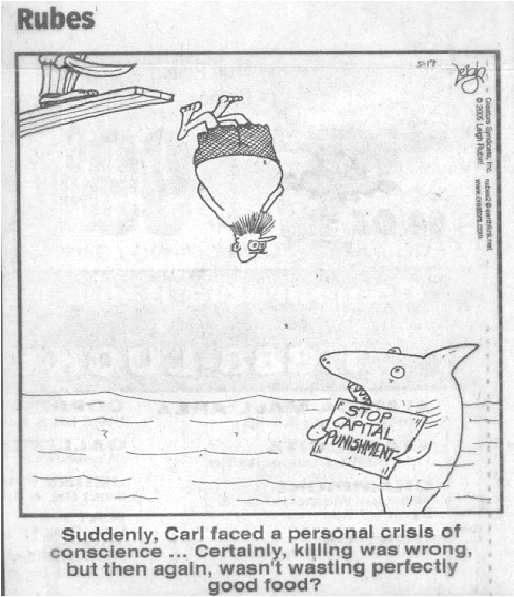
\includegraphics[width=5in]{./figures/CarlsDilemma.pdf} 
   \caption{Carl's dilemma -- Actually not a true dilemma, Carl has a third but in-obvious choice - he could carry the pirate to safety!}
   \label{fig:example}
\end{figure}

For instance if the rule is unjust, but everyone is forced to comply, then one can make the argument that
an unjust rule applied uniformly is fair.  However, the argument holds only if everyone is treated the same; otherwise we end up in the Orwellian situation that ''All pigs are equal, but some pigs are more equal than others.''  In practice rules are not applied uniformly, and thus dilemmas are common.  Taken to the extreme compliance might do more harm than good (consider the Katrina example regarding immediate survival)

\item Finally, benefit-cost analysis is fundamentally an application of utilitarianism. Costs of an action are usually straightforward to predict. Benefits require guess work; some benefits are not economically quantifiable.

Often only policy (politics) can assign benefit in these situations.  Like the more abstract points above, the question always arises (think of the pigs) \textsl{Are those who benefit the same as those who bear the costs?}  Consider taxation and public infrastructure - some fraction of our taxes goes to benefit people in South Dakota - how much benefit do we (bearing a portion the cost) receive?  Of course, they pay taxes that we spend, so there is at least in concept, some economic parity.
\end{enumerate}

So what is the point?  The point is that ethics is neither new nor well posed - there will always be conflicts and that is the purpose of the ethics component of continuing education.  The real goal is to identify when conflicts exist and provide us with a way to reason through them, and that reasoning needs to be based on value, duty, and utility and not just economic gain.  Also notice in the theories the unifying concepts of ''virtue'' and ''individual and common good.''